% !TEX root = ../../main.tex
%

\chapter{Background} \label{chap:background}
\section{Concurrency Control}

Concurrency control is a critical aspect of systems where multiple processes or threads access shared resources simultaneously, such as data structures, database tables, system resources etc. 
In general, concurrency control mechanisms utilize some form of synchronization to ensure safety and consistency of shared resources. 
According to \citet{DBLP:books/daglib/0030596}, synchronization is a set of rules and mechanisms that allows the specification and implementation of sequencing properties on statements issued by the processes so that all the executions of a multi-process program are correct. 

The form of synchronization studied in our work is \emph{competition synchronization} where multiple threads compete for access to shared resources. 
Locking is one of the primary mechanisms used to ensure data integrity and consistency in such environments.
For data-structures like lists, trees or graphs, locking involves restricting access to a data structure by multiple threads or processes to prevent conflicts and ensure that only one thread can modify the data at a time. Here’s a high-level overview of how locking works and its role in concurrency control:

% \subsection{Mutex (Mutual Exclusion) Locks}

% A mutex is a lock that ensures only one thread can access a resource at a time.
% When a thread acquires a mutex, other threads attempting to acquire the same mutex are blocked until the mutex is released.

% \begin{lstlisting}
%     std::mutex mtx;
%     int counter = 0;

%     void increment(int iterations) {
%         for (int i = 0; i < iterations; ++i) {
%             std::lock_guard<std::mutex> lock(mtx);
%             ++counter;
%         }
%     }
% \end{lstlisting}

% Mutex locks are simple and easy to implement but incur significant concurrency penalty due to the blocking nature of the lock. This can lead to performance degradation in scenarios where multiple threads contend for the same resource and should in theory be allowed to progress in parallel based on their operation. 


\subsection{Reader-Writer Locks}
Reader-writer locks, also called as shared-exclusive locks, are a type of lock that allows multiple threads to read a resource simultaneously but restrict write access to one thread at a time. This is useful when read operations are more frequent than write operations since a multiple readers can access the resource concurrently.

\begin{lstlisting}
    ReaderWriterLock rwlock;
    int counter = 0;

    void reader(int iterations) {
        for (int i = 0; i < iterations; ++i) {
            rwlock.reader_lock();
            // Read operation (e.g., print counter)
            std::cout << "Read counter: " << counter << std::endl;
            rwlock.reader_unlock();
        }
    }

    void writer(int iterations) {
        for (int i = 0; i < iterations; ++i) {
            rwlock.writer_lock();
            ++counter;
            rwlock.writer_unlock();
        }
    }
\end{lstlisting}

Read-write locks are more complex than simpler mutex locks but can improve performance in scenarios where read operations are more frequent than write operations. However, they can introduce additional complexity and potential issues like writer starvation where writers are blocked indefinitely by readers in the absence of proper fairness mechanisms.



% Spinlocks:
% \begin{lstlisting}
%     Spinlock spinlock;
%     int counter = 0;

%     void increment(int iterations) {
%         for (int i = 0; i < iterations; ++i) {
%             spinlock.lock();
%             ++counter;
%             spinlock.unlock();
%         }
%     }
% \end{lstlisting}
% Spinlocks are a type of lock where a thread repeatedly checks if the lock is available, consuming CPU cycles.
% They are useful in scenarios where the wait time is expected to be very short.
% Example in C++:
\subsection{Role of Locking in Concurrency Control}
\paragraph{Preventing Race Conditions}

Race conditions occur when multiple threads access and modify shared data concurrently, leading to unpredictable results.
Locks ensure that only one thread can modify the data at a time, preventing race conditions.

\paragraph{Ensuring Data Consistency}

Locks help maintain data consistency by ensuring that operations on shared data are atomic (indivisible).
This means that a series of operations can be completed without interruption, ensuring the data remains in a consistent state.

\paragraph{Deadlock Prevention}

Proper use of locks can help prevent deadlocks, where two or more threads are waiting indefinitely for each other to release locks.
Techniques like lock ordering and timeout mechanisms can be used to avoid deadlocks.


% Improving Performance:

% While locks can introduce overhead, they are essential for ensuring the correctness of concurrent programs.
% Using appropriate locking mechanisms (e.g., read-write locks) can help balance performance and data integrity.
% Example Scenario
% Consider a shared data structure like a linked list that multiple threads need to update:

% % In this example, the std::lock_guard ensures that the mutex is automatically released when the function exits, even if an exception is thrown.

% Conclusion
% Locking is a fundamental technique in concurrency control that helps ensure the integrity and consistency of shared data structures in multi-threaded environments. By understanding and correctly implementing locking mechanisms, you can prevent race conditions, maintain data consistency, and improve the overall reliability of your concurrent programs.


\section{Hierarchical data structures}
Hierarchical data models, rooted in the early days of computer science, have played a critical role in the representation and storage of structured information. 
The origins of hierarchical data can be traced back to the 1960s with the development of the Information Management System (IMS) by IBM \cite{IBMIMS}, which was one of the earliest database management systems designed for hierarchical data organization.  
IMS was created to manage the complex manufacturing data for the Apollo space program, establishing a clear, parent-child relationship between data entities, a key feature of hierarchical models \cite{DBLP:books/daglib/0006734}. 
Over the decades, hierarchical data structures have remained relevant, particularly in areas requiring nested or tree-like relationships, such as XML data management, file system hierarchies, and organizational charts \cite{DBLP:books/mk/BunemanSA99}. 
The importance of hierarchical models has been magnified in modern big data contexts, where they are often combined with other models (like graph databases) to handle the challenges posed by the complexity and interconnectedness of data. 
For example, hierarchical data models have been instrumental in NoSQL databases like Apache HBase, where efficient storage and quick retrieval of large-scale, semi-structured data are essential \cite{DBLP:books/daglib/0027893}. 
The structured nature of hierarchical models is well-suited for applications such as social networks, content management, and cloud-based storage systems, where data relationships are crucial. 
Thus, hierarchical data remains foundational to modern computing, providing a clear and efficient way to organize and retrieve complex, nested information. 

Formally, a hierarchy is defined as follows:

\begin{definition}
    A hierarchy is a directed graph H=(V,E) where
    \begin{itemize}
        \item V is a finite set of vertices
        \item $E \subset V \times V$ is a set of directed edges where each edge (u,v) represents a parent-child relationship between vertices u (the parent) and v (the child).
    \end{itemize} 
\end{definition}


\section{Locking in Hierarchical Data Structures}
Locking in hierarchical data structures is a crucial mechanism for ensuring data consistency and integrity, especially in concurrent environments where multiple processes or threads may attempt to access or modify the data simultaneously. 
Hierarchical data structures often require specialized locking techniques to efficiently manage concurrent access due to their inherently nested and dependent relationships between nodes. 
The goal of locking in these structures is to prevent race conditions, where two or more operations interfere with each other, potentially leading to incorrect data state. 

\subsection{Classical locking approaches in hierarchical data}
A common approach is lock coupling \cite{BayerS77}, also known as hand-over-hand locking, where a thread locks a vertex before traversing to one of its children in the hierarchy, unlocking the parent once the child is locked. 
This allows for fine-grained synchronization, which improves concurrency by permitting multiple threads to work on different parts of the hierarchy simultaneously. 
However, \citet{LeisH019} show that lock coupling can lead to suboptimal locking performance on modern hardware. 


An alternative to lock coupling is a B-Tree variant called B-Link tree \cite{LehmanY81} in which, a thread holds a single lock at time with optimistic reachability checks. 
However, for in-memory workloads, B-Link trees suffer from the same performance issues as lock coupling.

Classical locking techniques for hierarchical data structures are often designed with a synchronization hypothesis. 
Their design limits their use in general purpose applications where the topology of the hierarchy is not known a priori. 

\subsection{Fixed Grain locking}
As an alternative of the classical approaches, reader-writer locks are appropriated for hierarchical data by associating a lock with a predefined granularity. 
We refer to this as \emph{fixed grain locking}. 
Fixed grain locking has two extremes: We can either have a single lock for the entire hierarchy (coarse grain locking) or a lock for each vertex (fine grain locking).
% The granularity of a lock determines the degree of concurrency and the amount of contention in the system. 



\begin{figure}[H]
    \captionsetup{justification=centering}
    \centering
    \begin{subfigure}{.49\textwidth}
        \centering
        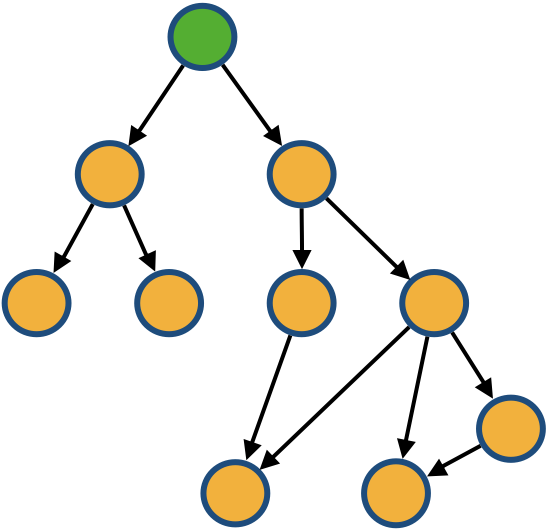
\includegraphics[width=.7\columnwidth]{figures/CoarseGrainedLockingTree}
        \caption{Coarse grain lock in a hierarchy.}        
        \label{fig:fixedLockGrainsCoarse}
    \end{subfigure}
    \begin{subfigure}{.49\textwidth}
        \centering
        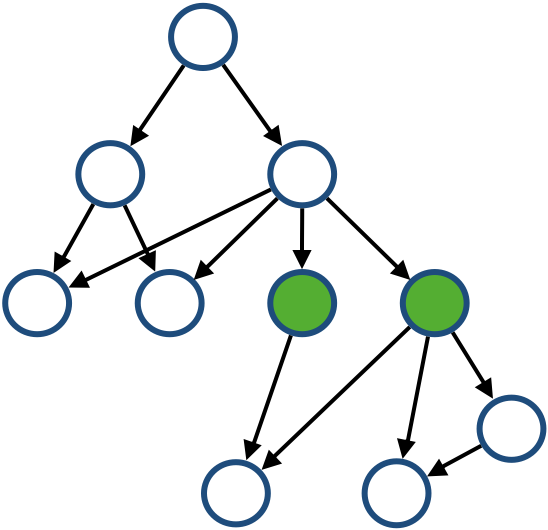
\includegraphics[width=.7\columnwidth]{figures/FineGrainLockingTree}
        \caption{Fine grain locks in a hierarchy.}
        \label{fig:fixedLockGrainsFine}
    \end{subfigure}
    
    \label{fig:fixedLockGrains}
\caption{Fixed grain locking in hierarchical data structures (lock guard in green and the corresponding grain in yellow).}
\end{figure}


\paragraph{Coarse Grain Locking}
An oversimplified approach to correctness is to guard the root of the hierarchy such that any thread accessing the hierarchy must first acquire the root lock.
This approach is called \emph{coarse grain locking} and is shown in Figure \ref{fig:fixedLockGrainsCoarse}.
A thread that wishes to access any vertex in the hierarchy must first acquire the root lock and consequently block all other writers until it releases this lock. 
Coarse grain locking is simple to implement and has extremely low locking overhead but suffers from the highest possible contention as all threads must acquire the same lock to access any part of the hierarchy. 


\paragraph{Fine Grain Locking}
Another well known approach to locking is when every target vertex is its own guard i.e. every vertex has its own lock. 
We call this \emph{fine grain locking}.
As shown in Figure \ref{fig:fixedLockGrainsFine}, the vertices are locked individually and a thread that needs to access multiple vertices must acquire multiple locks. 
Fine grain locking has the advantage of reducing contention as threads can access disjoint parts of the hierarchy concurrently. 
However, the overhead of acquiring multiple locks makes this approach less efficient. 


\subsection{Multi-Granularity Locking}
An alternative approach to locking in hierarchical data structures is multiple granularity locking, which adapts the granularity of locks based on the structure of the hierarchy. 
According to \citet{gray1975granularity}, hierarchical or multi-granularity locking involves locking a vertex in a hierarchy such that the lock is sufficient to protect the vertex and its descendants i.e. a thread that requests a write (exclusive) lock on a vertex implicitly exclusively locks all its descendants when its request is granted. 

A vertex which a thread intends to access is called the \emph{lock target} of the thread. 
MGL methods generally associate a lock with each vertex in the hierarchy which we call the \emph{guard} of the vertex. 
As such, when a thread wishes to access a target, it must acquire an appropriate lock on the guard of the the target vertex. 



The approaches shown in Figures \ref{fig:fixedLockGrainsFine} and \ref{fig:fixedLockGrainsCoarse} have their own trade-offs. 
Coarse grain locking causes unnecessary contention by blocking threads that access disjoint parts of the hierarchy. 
Fine grain locking, on the other hand, introduces significant overhead due to the need to acquire multiple locks for accessing multiple vertices with the additional requirement of deadlock detection and prevention.


\emph{Multi-granularity locking} (MGL) \cite{gray1975granularity} techniques find a balance between the two extremes by identifying a theoretically optimal lock guard for a given target based on the topology of the hierarchy.
% \emph{Multi-granularity locking} (MGL) \cite{gray1975granularity} techniques exploit the topology of the graph to identify a pertinent guard for a given target and aim to strike a balance between these two extremes. 
Since grain size (the \emph{granularity}) depends on the topology of the graph and on the lock request, different lock requests have different granularities, hence the name.

\begin{figure}[h]
    \captionsetup{justification=centering}
    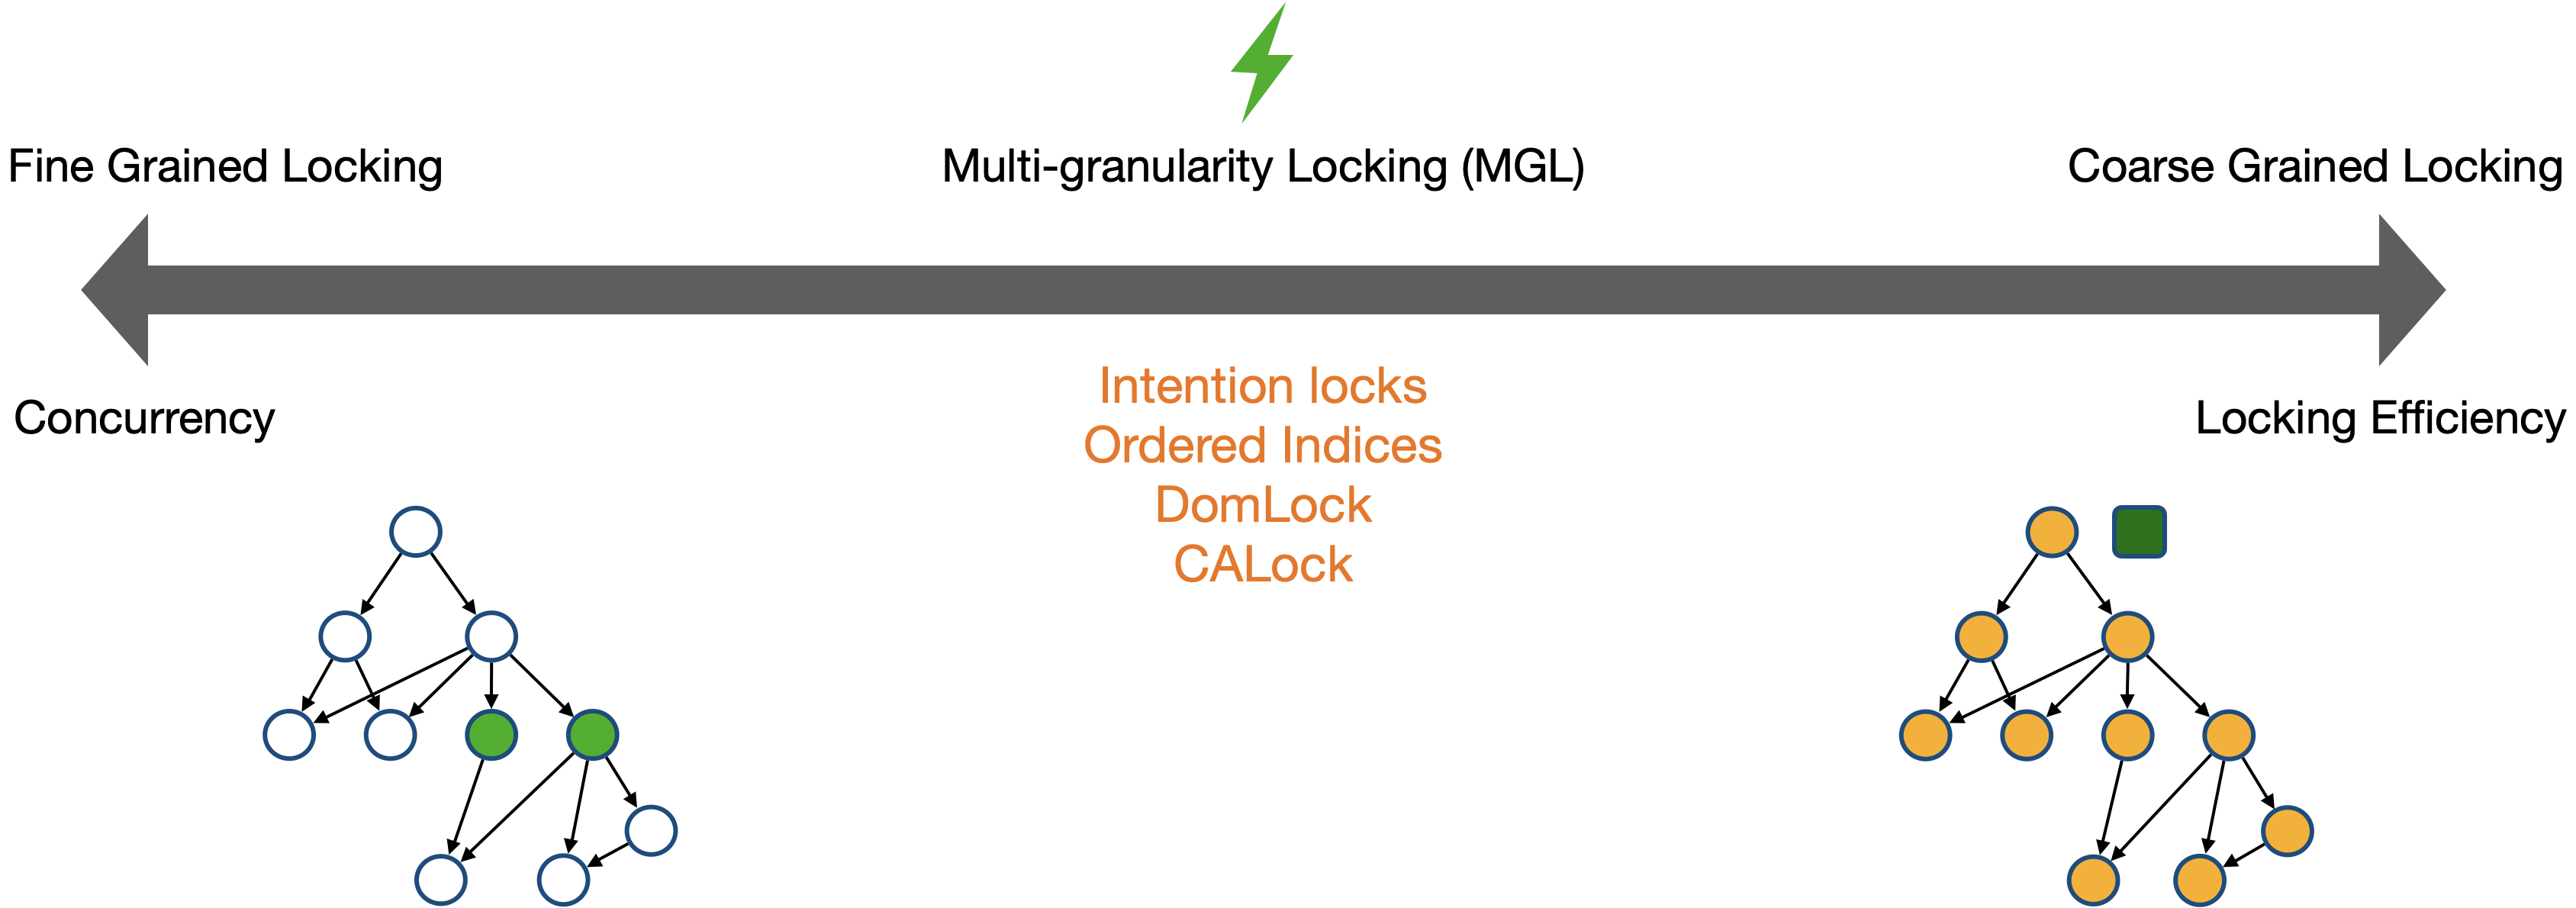
\includegraphics[width=\textwidth]{figures/MGLSpectrum.png}
    \label{fig:mglspectrum}
    \caption{Multi-Granularity locking provides a balance between Fine grain and Coarse grain locking.}
\end{figure}

A classical example of MGL is \emph{Intention locks} \cite{StonebrakerGranularity} which are often used in database indices to optimize hierarchical access \cite{sqlintentionlocks}. 

Another dimension of complexity with hierarchical data is the mutation of the hierarchy itself which causes topological changes.
We refer to to such mutations as \emph{structural modifications}.

Although there already exist effective MGL algorithms for graphs that do not undergo structural modifications, this is not the case for graphs whose structure can mutate. 
We discuss this in Chapter \ref{chap:relatedwork}.
A structural modification operation adds or removes vertices and{\slash}or edges and may conflict with ordinary operations, or with another structural modification.
Such operations affect the identification of lock granules as their size and shape now depend on the new topology of the graph.



% \section{Related Work}
% Survey of existing research on locking mechanisms and optimization techniques. Comparison of related approaches to the CALock algorithm.

\section{Context}
This work on locking focusses on a multi-core system where threads concurrently access a shared graph. Such use-cases, prevalent as graph processing applications, provide the possibility to use a single centralized scheduler which decides on the ordering of the lock requests. In distributed deployments like HPC clusters where the communication can be guaranteed to be quasi-instantaneous, locking can still be useful. Geo-distributed graphs and synchronization are out of the scope of this work. As such, locking in any form is not an efficient solution for use-cases where the graph is geo-distributed and the communication latency (ergo the synchronization delay) is high. 

The requirement for any locking technique over graphs is to protect the vertices and edges of the graph against concurrent write access. Writes can modify the data on the vertices or add/remove edges from the graph. A application that uses CALock can have multiple threads that concurrently access the graph. Each thread can request a lock on a set of vertices(lock targets). The locking algorithm then grants the lock request by locking a single vertex(the guard), that protects the set of vertices.
Once a thread identifies a guard and issues a lock request, the guard cannot to be changed i.e. the guard is fixed for the duration of the lock. This is to ensure that the lock grain remains consistent for the duration of the lock. If a conflict is detected between two lock requests, one of the threads is blocked until it is notified to resume i.e. no busy waiting. 

In our design, we assume that the threads are not malicious and do not try to circumvent the locking and conflict detection mechanism
